\documentclass{standalone}
\usepackage{tikz}
\usepackage{amsfonts}
\usetikzlibrary{calc}
\usetikzlibrary{intersections}

%% Document
\begin{document}

	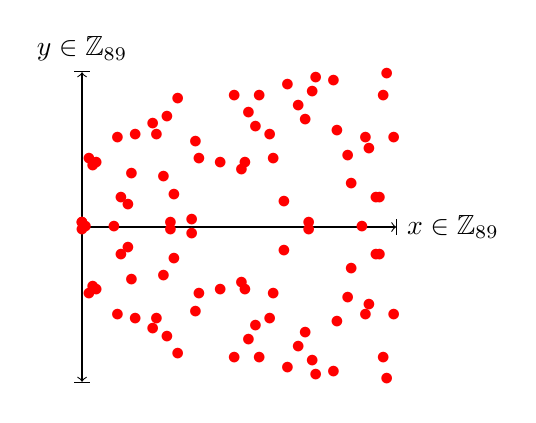
\begin{tikzpicture}[scale=.045]

      \draw[|<->|,black] (0,-44) -- (0,44) node[above] {$y \in \mathbb{Z}_{89}$};
      \draw[->|,black] (0,0) -- (89,0) node[right] {$x \in \mathbb{Z}_{89}$};
      \foreach \point in {
        (0, 1), (0, 1), (0, -1), (1, 0), (2, 19), (2, -19), (3, 17), (3, -17), (4, 18), (4, -18), (9, 0),
        (10, 25), (10, -25), (11, 8), (11, -8), (13, 6), (13, -6), (14, 15), (14, -15), (15, 26), (15, -26),
        (20, 29), (20, -29), (21, 26), (21, -26), (23, 14), (23, -14), (24, 31), (24, -31), (25, 1), (25, -1), (26, 9), (26, -9), (27, 36), (27, -36),
        (31, 2), (31, -2), (32, 24), (32, -24), (33, 19), (33, -19), (39, 18), (39, -18),
        (43, 37), (43, -37), (45, 16), (45, -16), (46, 18), (46, -18), (47, 32), (47, -32), (49, 28), (49, -28),
        (50, 37), (50, -37), (53, 26), (53, -26), (54, 19), (54, -19), (57, 7), (57, -7), (58, 40), (58, -40),
        (61, 34), (61, -34), (63, 30), (63, -30), (64, 1), (64, -1), (65, 38), (65, -38), (66, 42), (66, -42),
        (71, 41), (71, -41), (72, 27), (72, -27), (75, 20), (75, -20), (76, 12), (76, -12), (79, 0),
        (80, 25), (80, -25), (81, 22), (81, -22), (83, 8), (83, -8), (84, 8), (84, -8), (85, 37), (85, -37), (86, 43), (86, -43), (88, 25), (88, -25)
      } {\node[red] at \point {$\bullet$};}

	\end{tikzpicture}

\end{document}
